% Appendix Template
\chapter{Appendix} % Main appendix title
\label{appA} % Change X to a consecutive letter; for referencing this appendix elsewhere, use \ref{AppendixX}
\begin{figure}[tbh!]
\centering
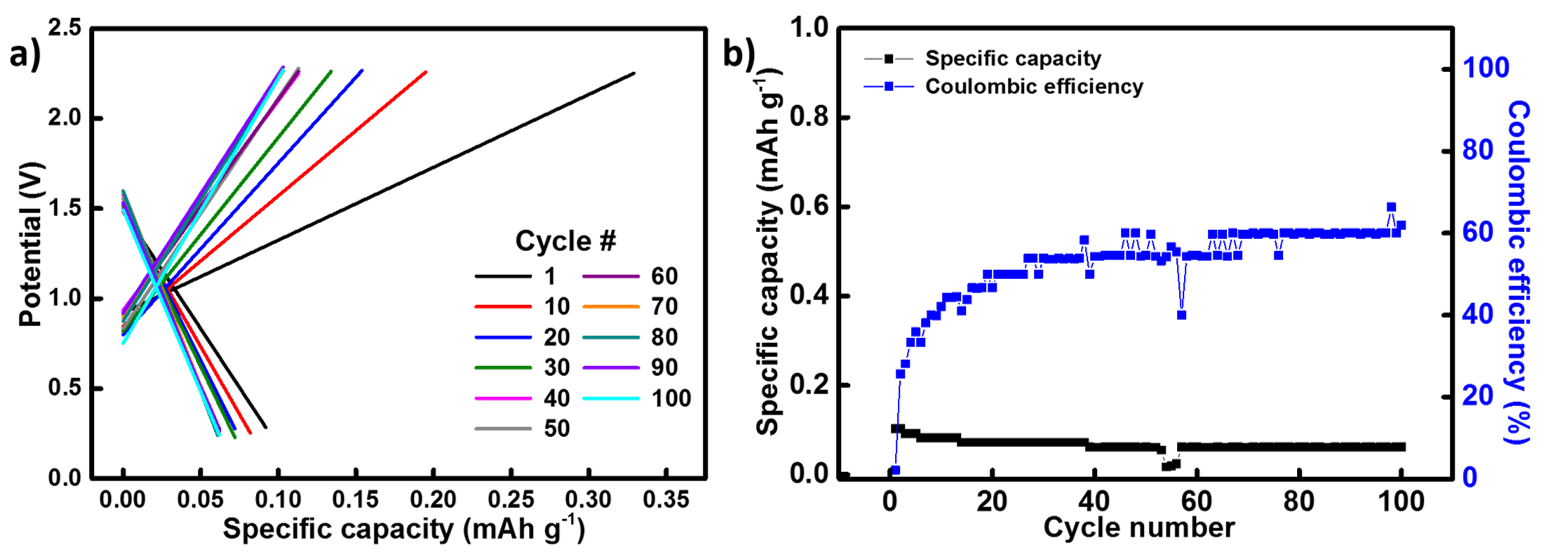
\includegraphics[width=\textwidth]{Figures/appendix/blankmo}
\caption{a) Galvanostatic charge/discharge curves of an Al/Mo cell using a two-electrode setup at a current rate of 40 mA g$^{-1}$. The cell failed to achieve any significant discharge capacities during both charge and discharge. b) Blank Mo foil displayed CE at 40\%. This confirmed that when acting as the current collector, molybdenum did not contribute any capacity of its own.}
\label{Figures/appendix:blankmol}
\end{figure}
\begin{figure}[tbh!]
\centering
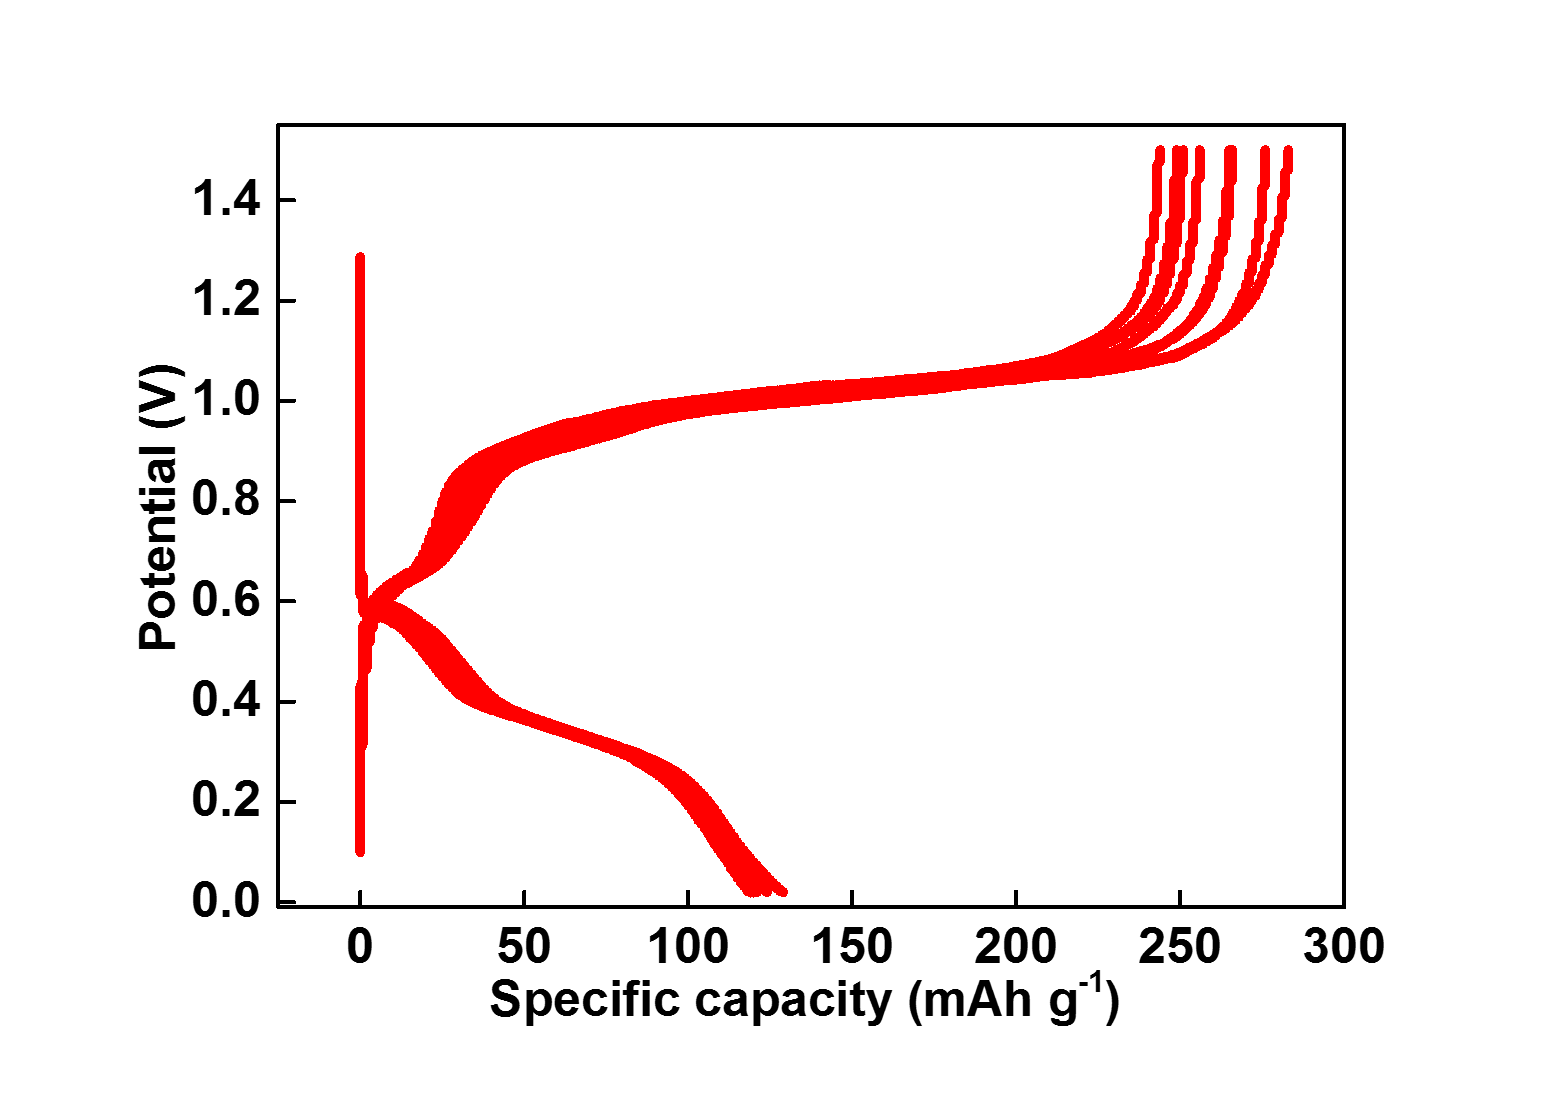
\includegraphics[width=\textwidth]{Figures/appendix/hBNrepeat}
\caption{Galvanostatic charge/discharge curves of Al/old h-BN cells using a two-electrode setup at a current rate of 40 mA g$^{-1}$. The cell achieved discharge capacities of 125 mAh g$^{-1}$ with plateau observed during discharge at 0.4 V. and a charging voltage at 1.0 V.}
\label{Figures/appendix:hBNrepeat}
\end{figure}
The figure below presents the data that was collected using \rq pouch cells\lq\ in Fraunhofer Institute, Dresden, Germany. A pouch cell contains conductive foil-tabs, made of nickel and aluminium, which were welded to both the electrodes and sealed completely inside a glove box. The pouch cell offers a simple, flexible and lightweight solution to battery design. The pouch cell makes most efficient use of space and achieves 90–95\% packaging efficiency, the highest among battery packs such as coin cells, Swagelok-type cells, cylindrical cells, etc.
\begin{figure}[tbh!]
\centering
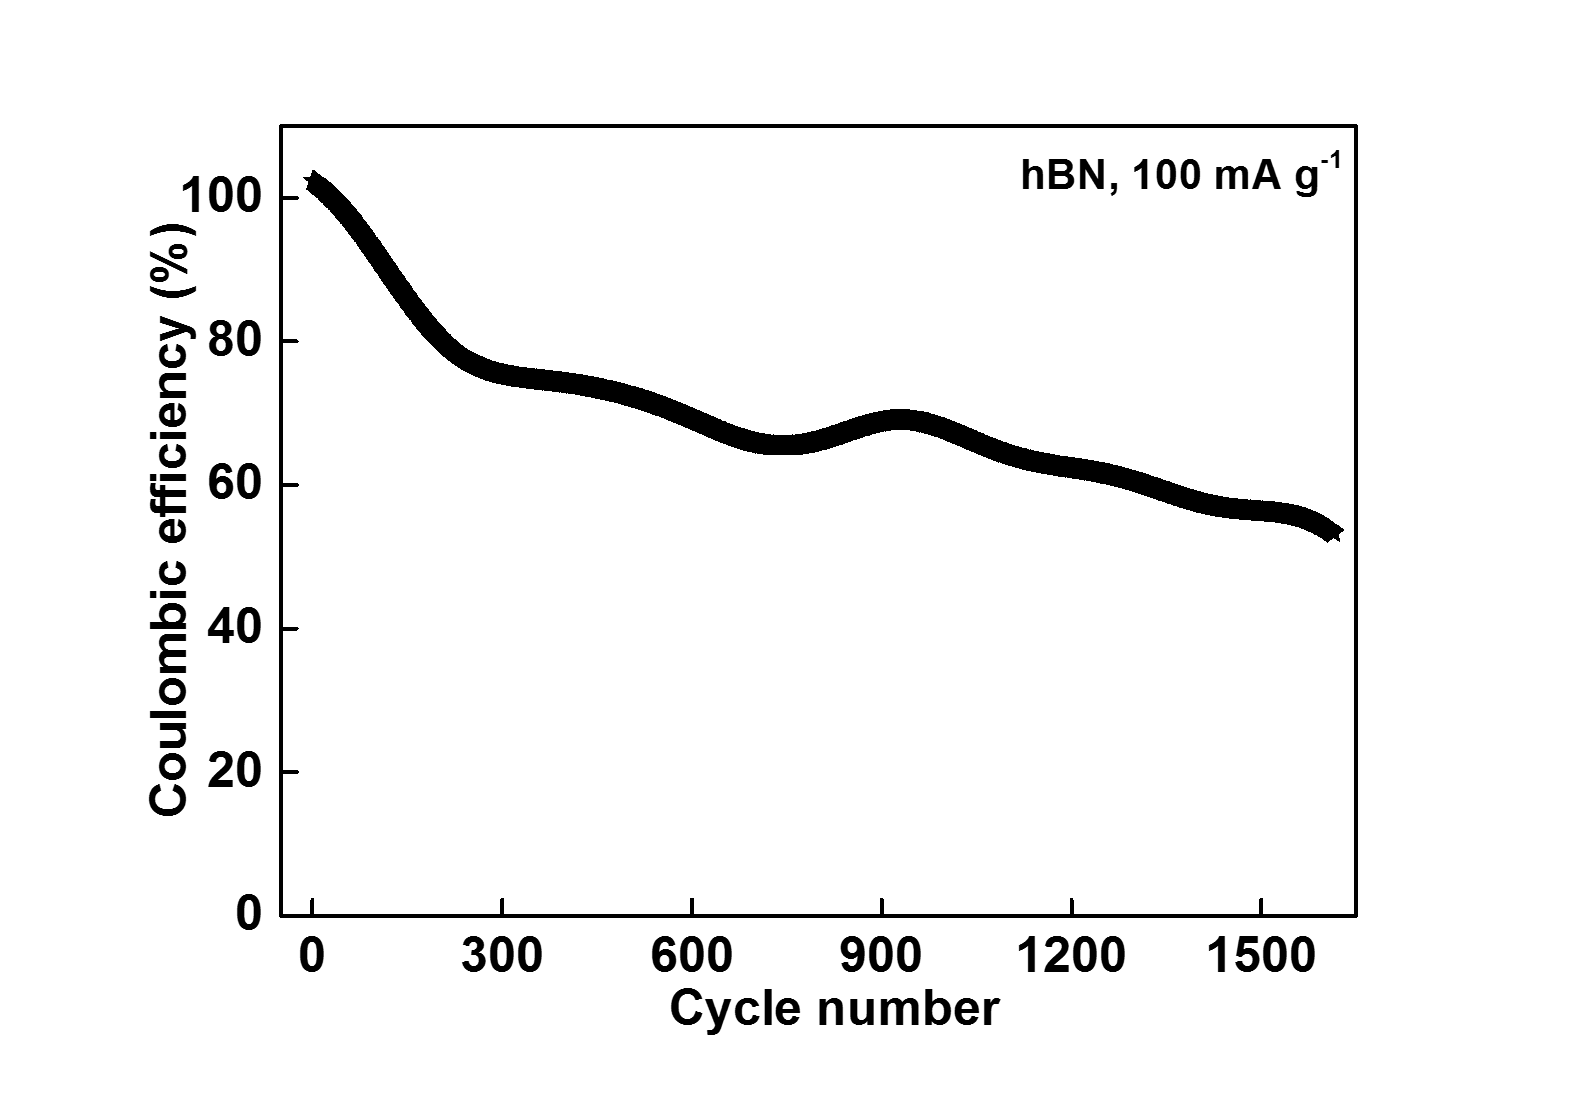
\includegraphics[width=\textwidth]{Figures/appendix/pouchCE}
\caption{a) Coulombic efficiency recorded for 1600 cycles of Al/old-hBN pouch cells assembled in IKTS, Germany.}
\label{Figures/appendix:pouchCE}
\end{figure}

\begin{figure}[tbh!]
\centering
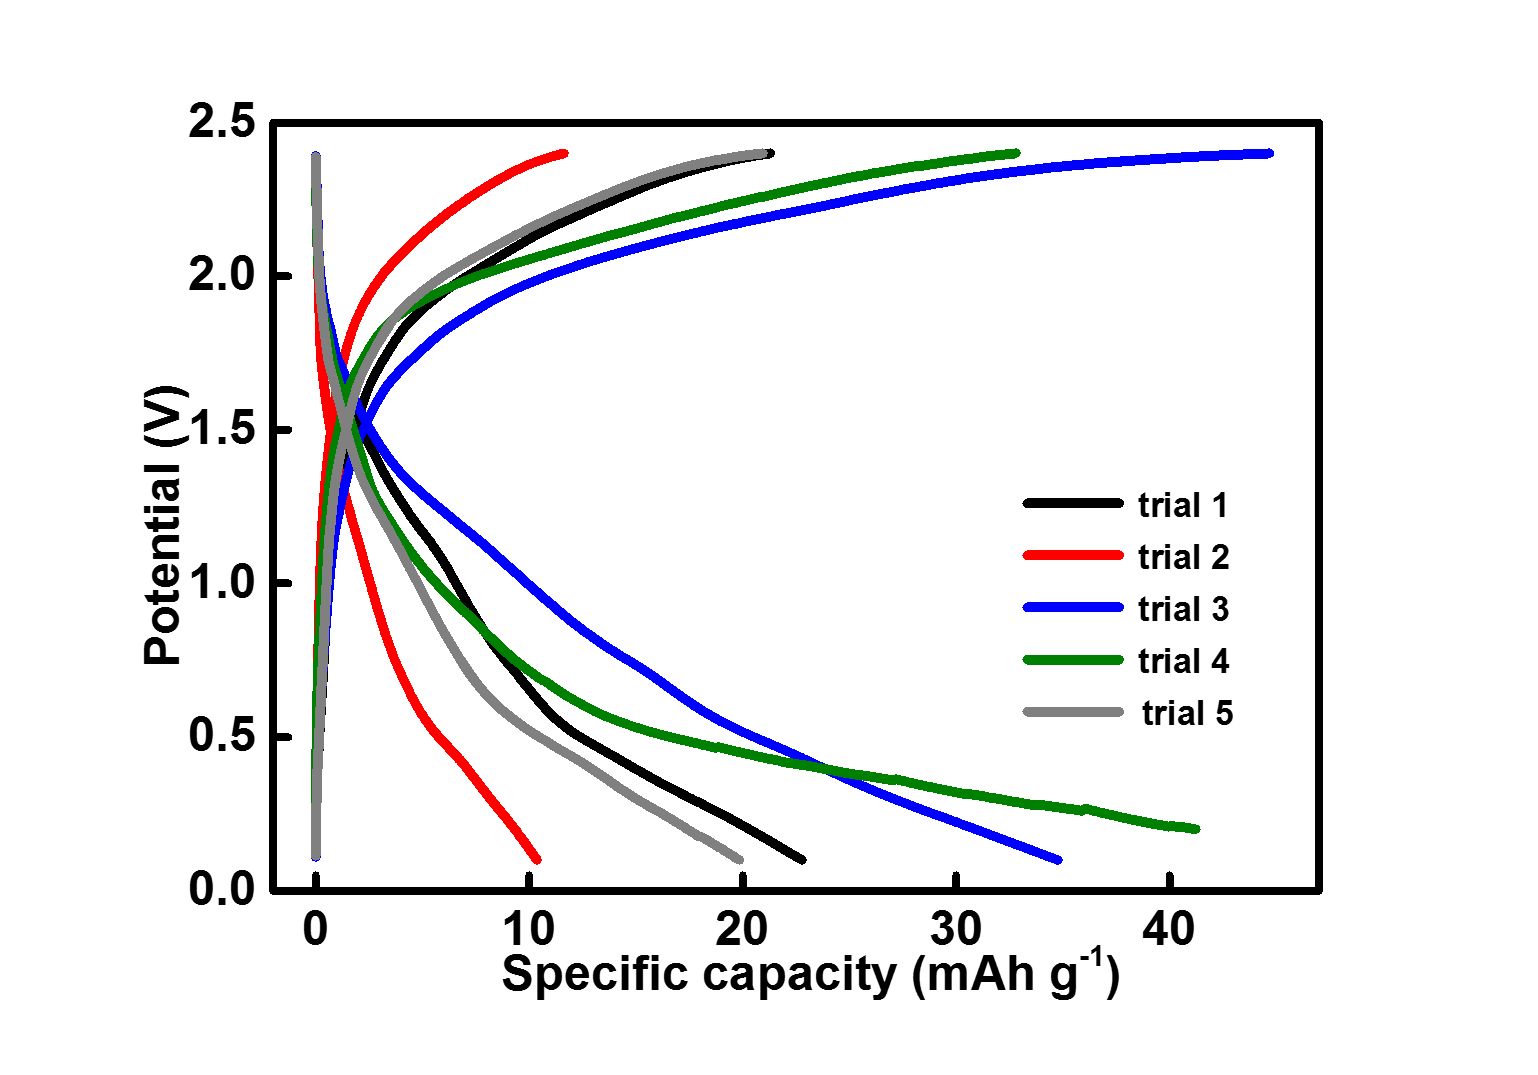
\includegraphics[width=\textwidth]{Figures/appendix/hBNmultiattempts}
\caption{CDCs of Al/hBN cells using pure hBN, 98\% pure, $\approx$1 $\mu$m in size using similar assembly conditions. All cells were run at a current rate of 40 mA g$^{-1}$. Despite repeated attempts, none of the cells recorded a capacity above 50 mAh g$^{-1}$. This was an issue because we were trying to replicate our previous results where an Al/hBN cells recorded capacities above 100 mAh g$^{-1}$, Figure \ref{Figures/appendix:hBNrepeat}.}
\label{Figures/appendix:hBNmultiattempts}
\end{figure}

\begin{figure}[tbh!]
\centering
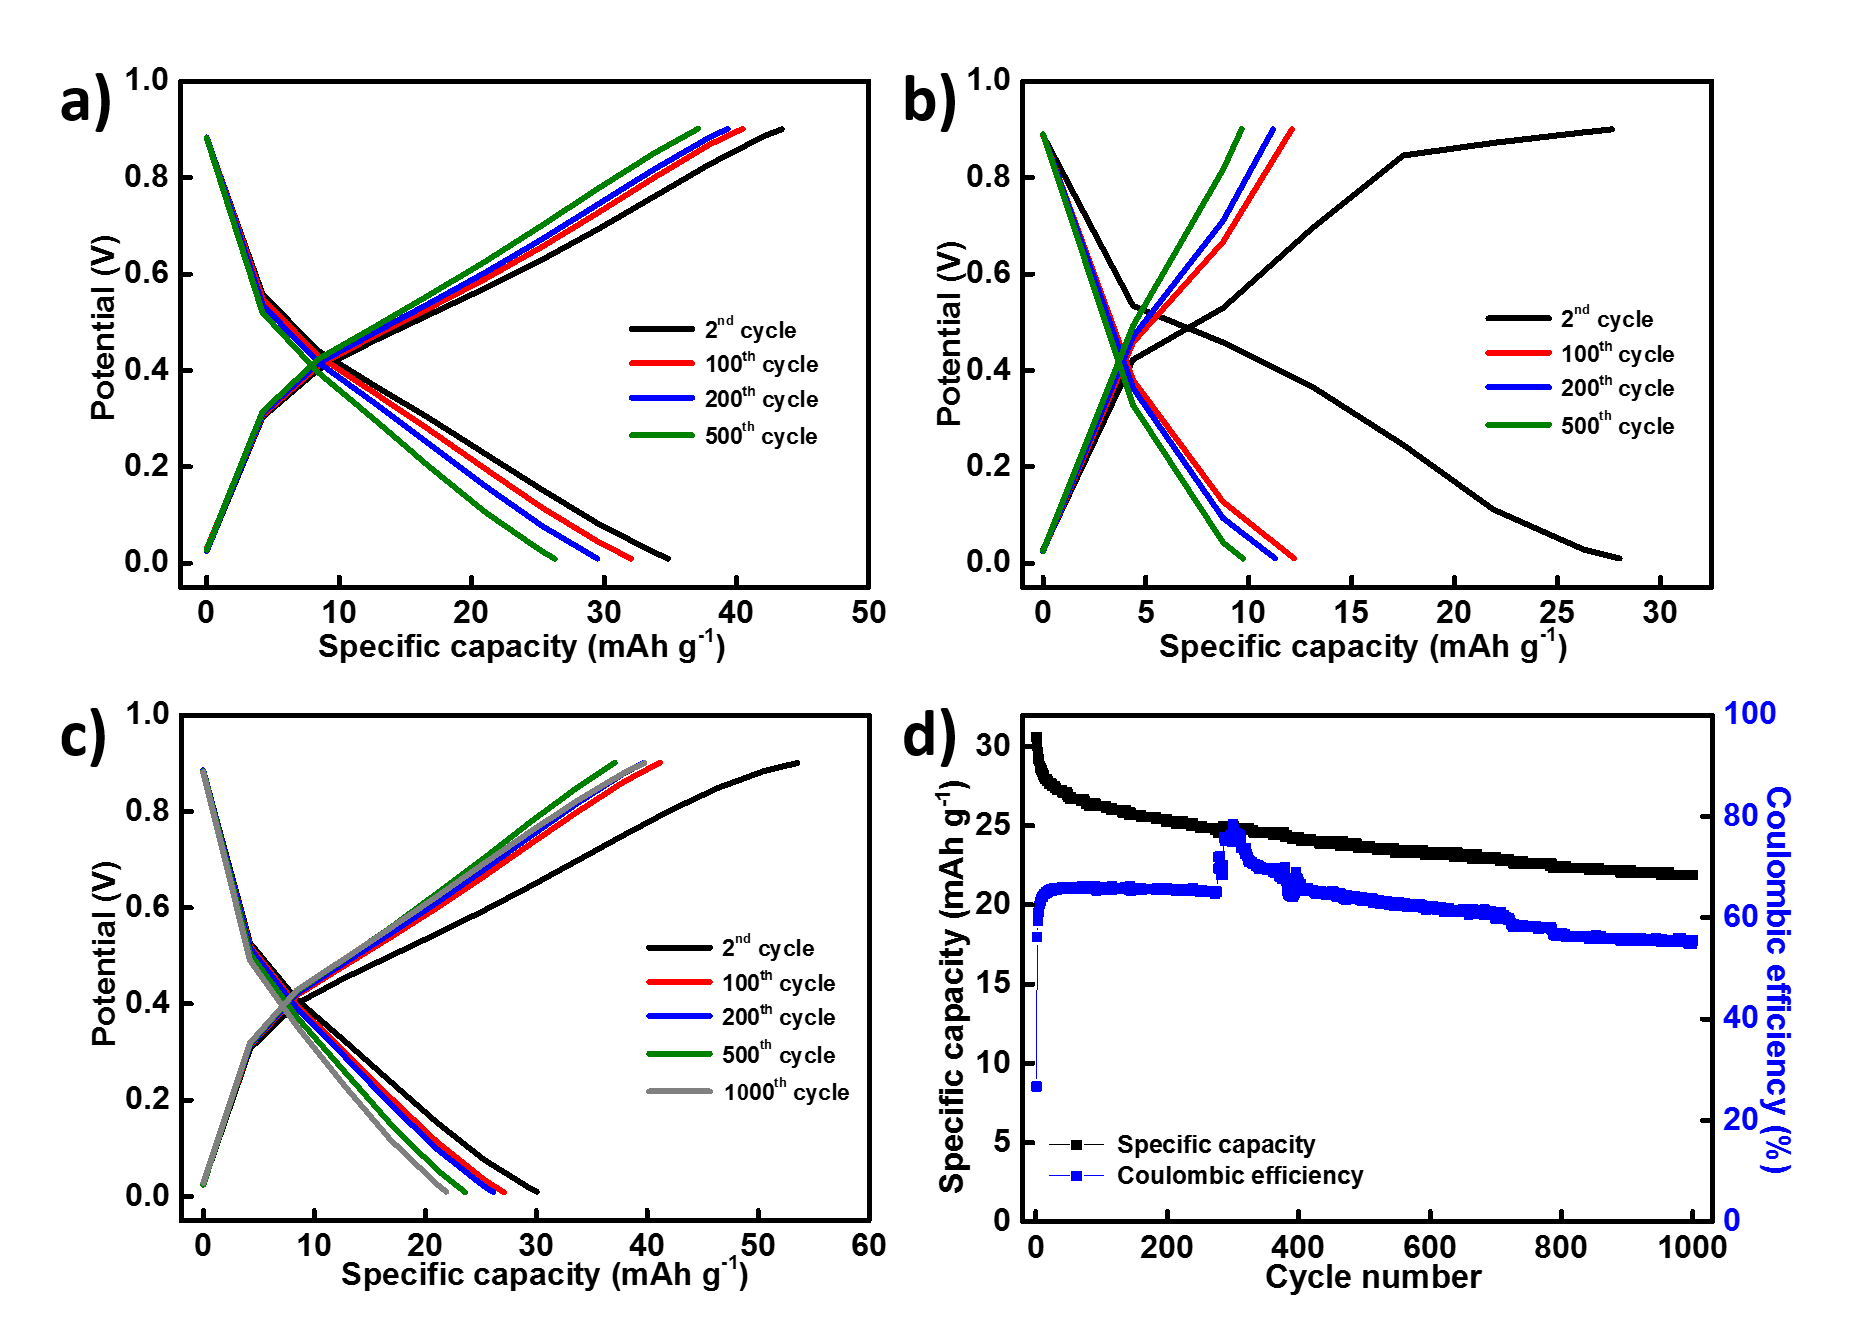
\includegraphics[width=\textwidth]{Figures/appendix/pouchcellCDCCE}
\caption{a-c) Cell performance of various Al/hBN pouch cells assembled in ITKS, Germany. None of the cells managed to achieve capacities above 50 mAh g$^{-1}$. d) Coulombic efficiency of an Al/hBN cell run for thousand cycles at a current rate of 40 mA g$^{-1}$. }
\label{Figures/appendix:pouchcellCDCCE}
\end{figure}
\begin{figure}[tbh!]
\centering
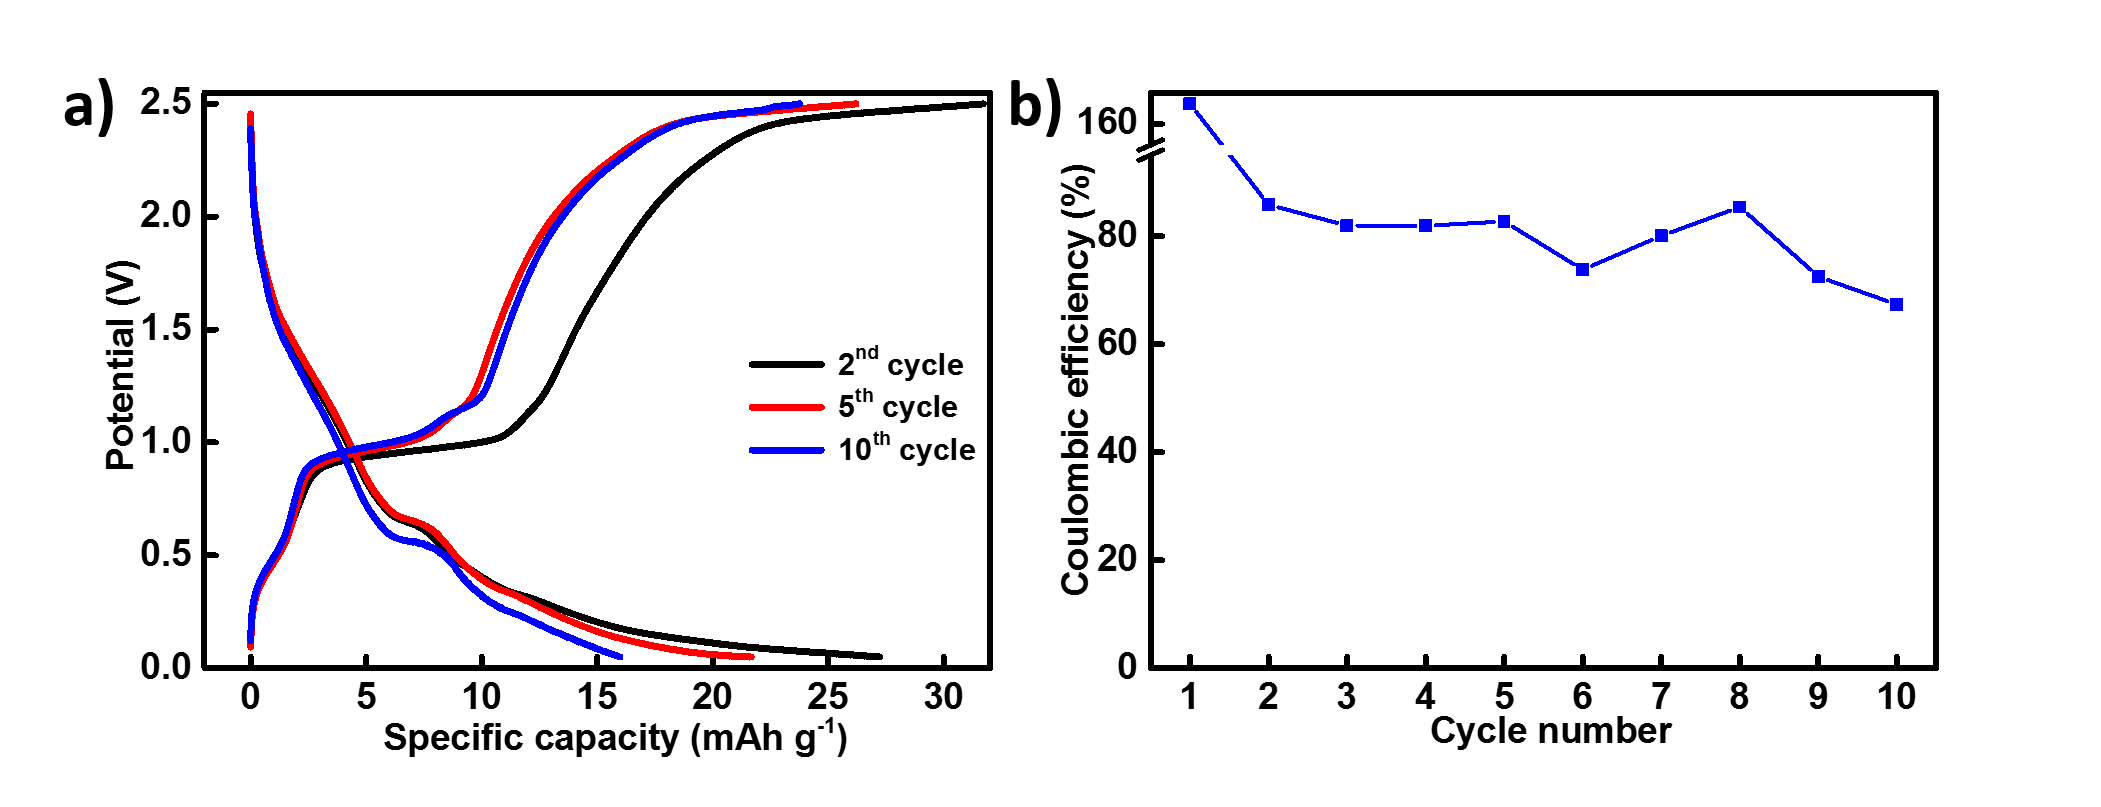
\includegraphics[width=\textwidth]{Figures/appendix/WS2CDCCE}
\caption{ a) Galvanostatic charge/discharge cycles, and b) coulombic efficiency of an Al/\ce{WS2} cell for 10 cycles at a current rate of 50 mA g$^{-1}$. A distinct plateau was seen during discharge at 0.68 V and a charging plateau was observed at 1.0 V vs \ce{Al$^{3+}$}/Al. \ce{WS2} has a layered structure similar to \ce{MoS2} with an interlayer distance of 6.18 \AA. Looking at the CDCs, a few \ce{AlCl4-} ions manage to intercalate but it seems the side reactions taking place at the electrode/electrolyte interface prevent the cell from achieving high specific capacities.}
\label{Figures/appendix:WS2CDCCE}
\end{figure}
\begin{figure}[tbh!]
\centering
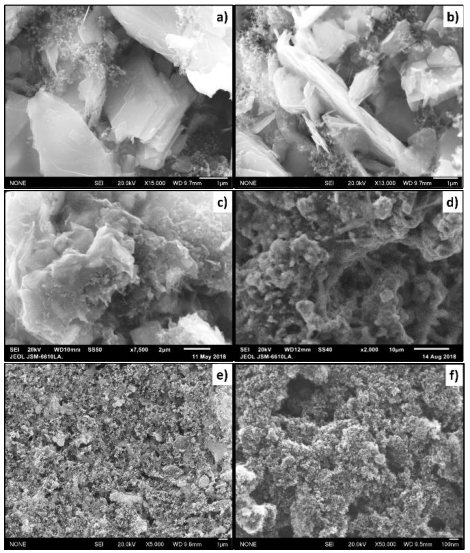
\includegraphics[width=\textwidth]{Figures/appendix/mox2sem}
\caption{SEM images of pristine a) \ce{MoS2} and b) \ce{MoSe2}; and cycled c) \ce{MoS2} and d) \ce{MoSe2}. SEM images of e) pristine and f) cycled MoSSe. \ce{MoS2} and \ce{MoSe2} clearly have a layered structure, while MoSSe lacks a long-range order.}
\label{Figures/appendix:semmox2cnt}
\end{figure}
\begin{figure}[tbh!]
\centering
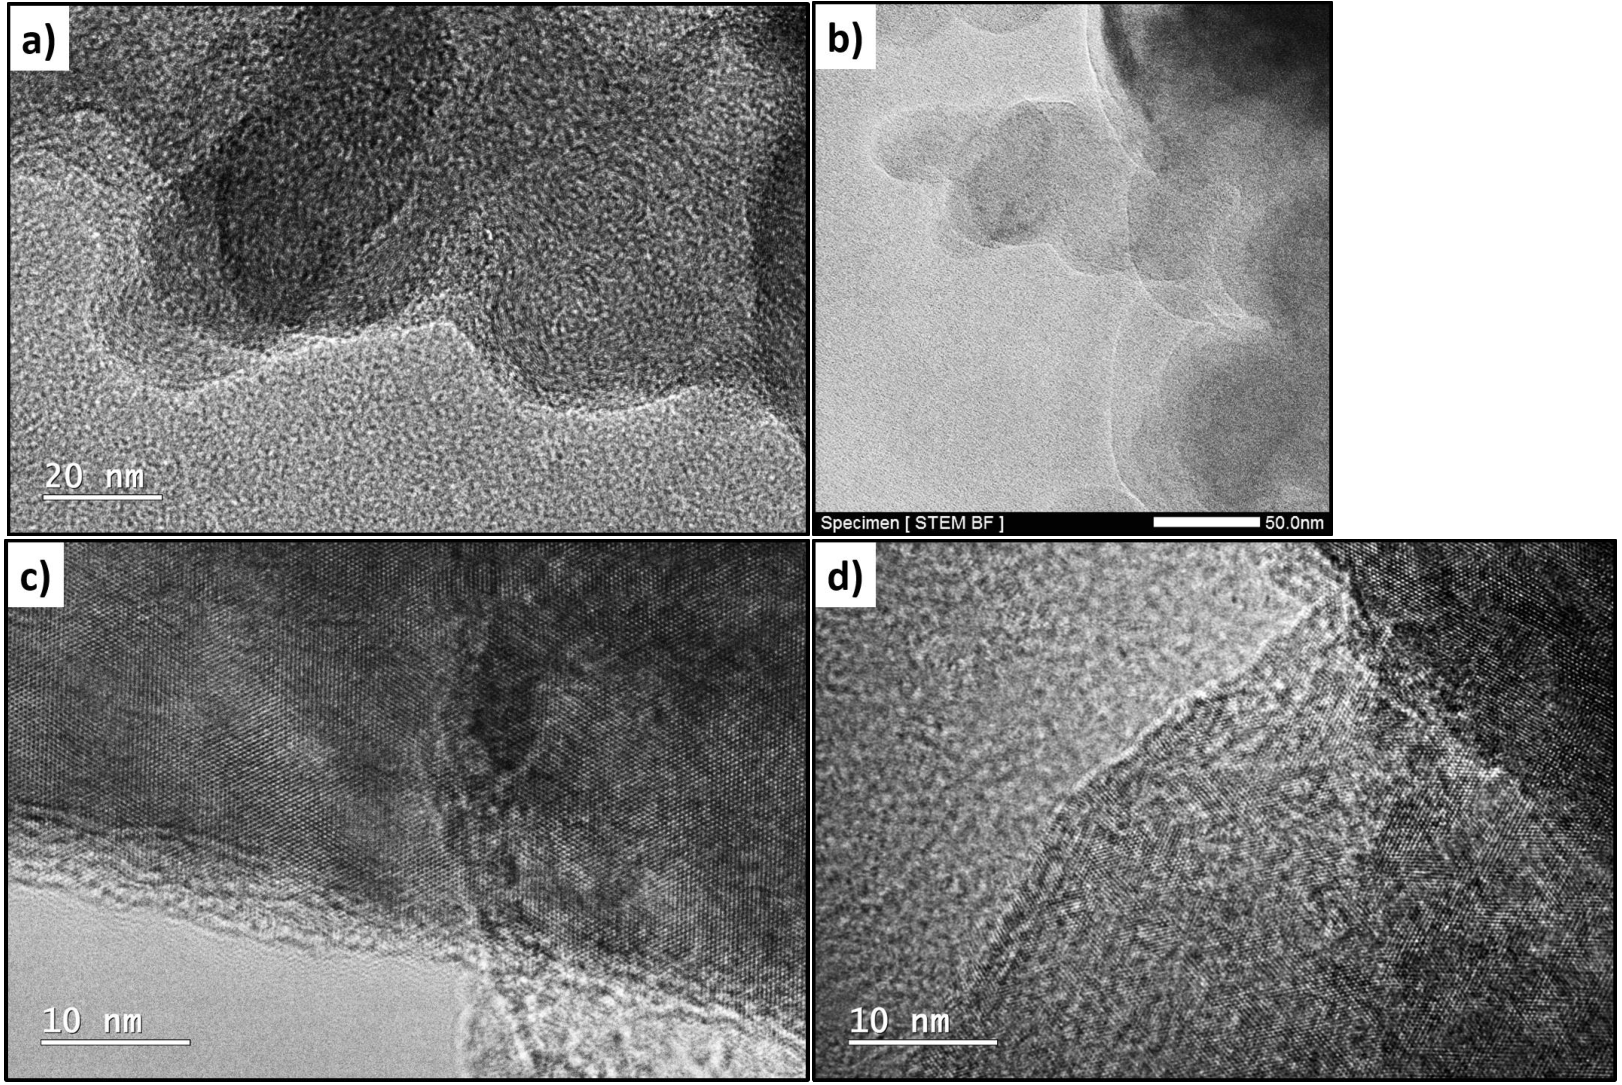
\includegraphics[width=\textwidth]{Figures/appendix/mox2tem}
\caption{TEM micrographs of a-b) pristine \ce{MoS2}, and c-d) \ce{MoSe2}. a and b display the presence of layered structure of \ce{MoS2}, c and d display the presence of multiple lattice fringes.}
\label{Figures/appendix:mox2tem}
\end{figure}
\begin{figure}[tbh!]
\centering
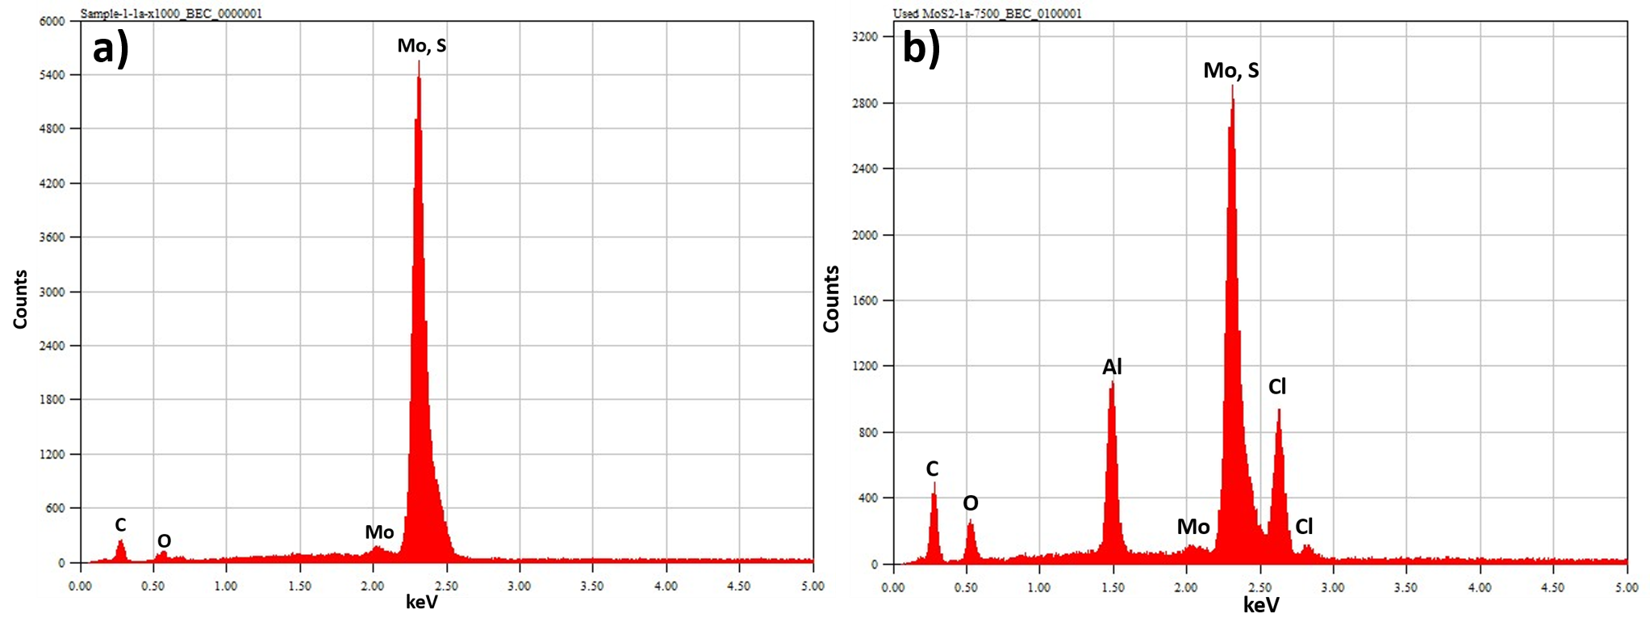
\includegraphics[width=\textwidth]{Figures/appendix/mos2edxpt}
\caption{Energy-dispersive X-ray spectroscopy (EDXS) profiles of a) pristine \ce{MoS2} and b) cycled \ce{MoS2} cathode. The cycled cathode shows presence of aluminium and chlorine in its spectra.}
\label{Figures/appendix:mos2edxpt}
\end{figure}
\begin{figure}[tbh!]
\centering
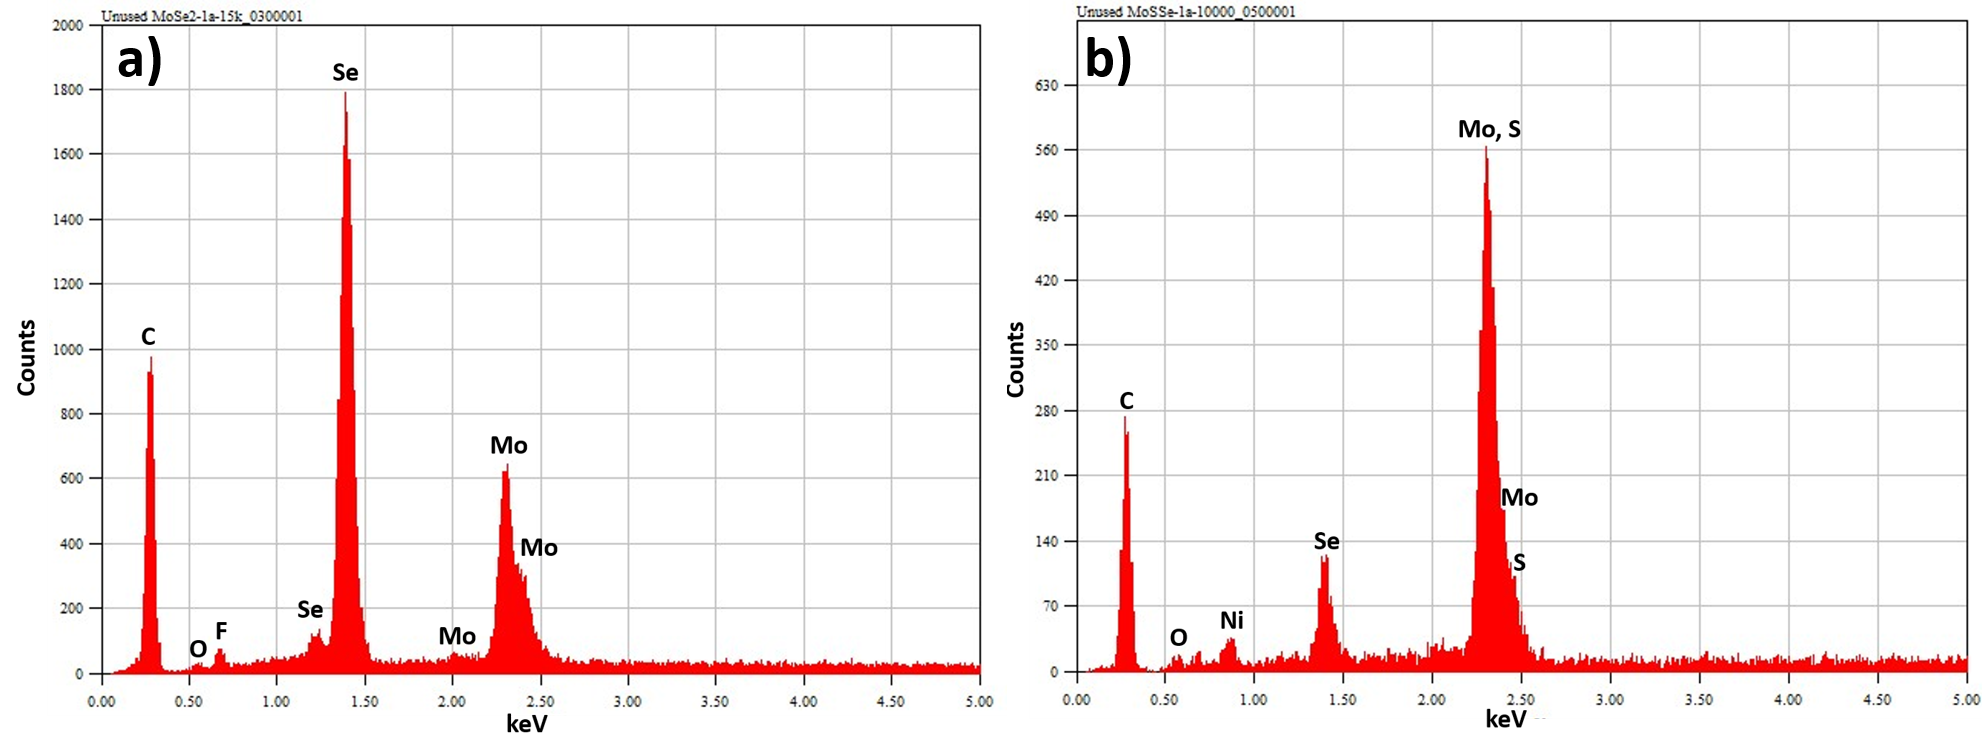
\includegraphics[width=\textwidth]{Figures/appendix/mose2mosseprt}
\caption{EDXS profiles of a) pristine \ce{MoSe2} and b) MoSSe. }
\label{Figures/appendix:mose2mosse}
\end{figure}
\begin{figure}
  \centering
  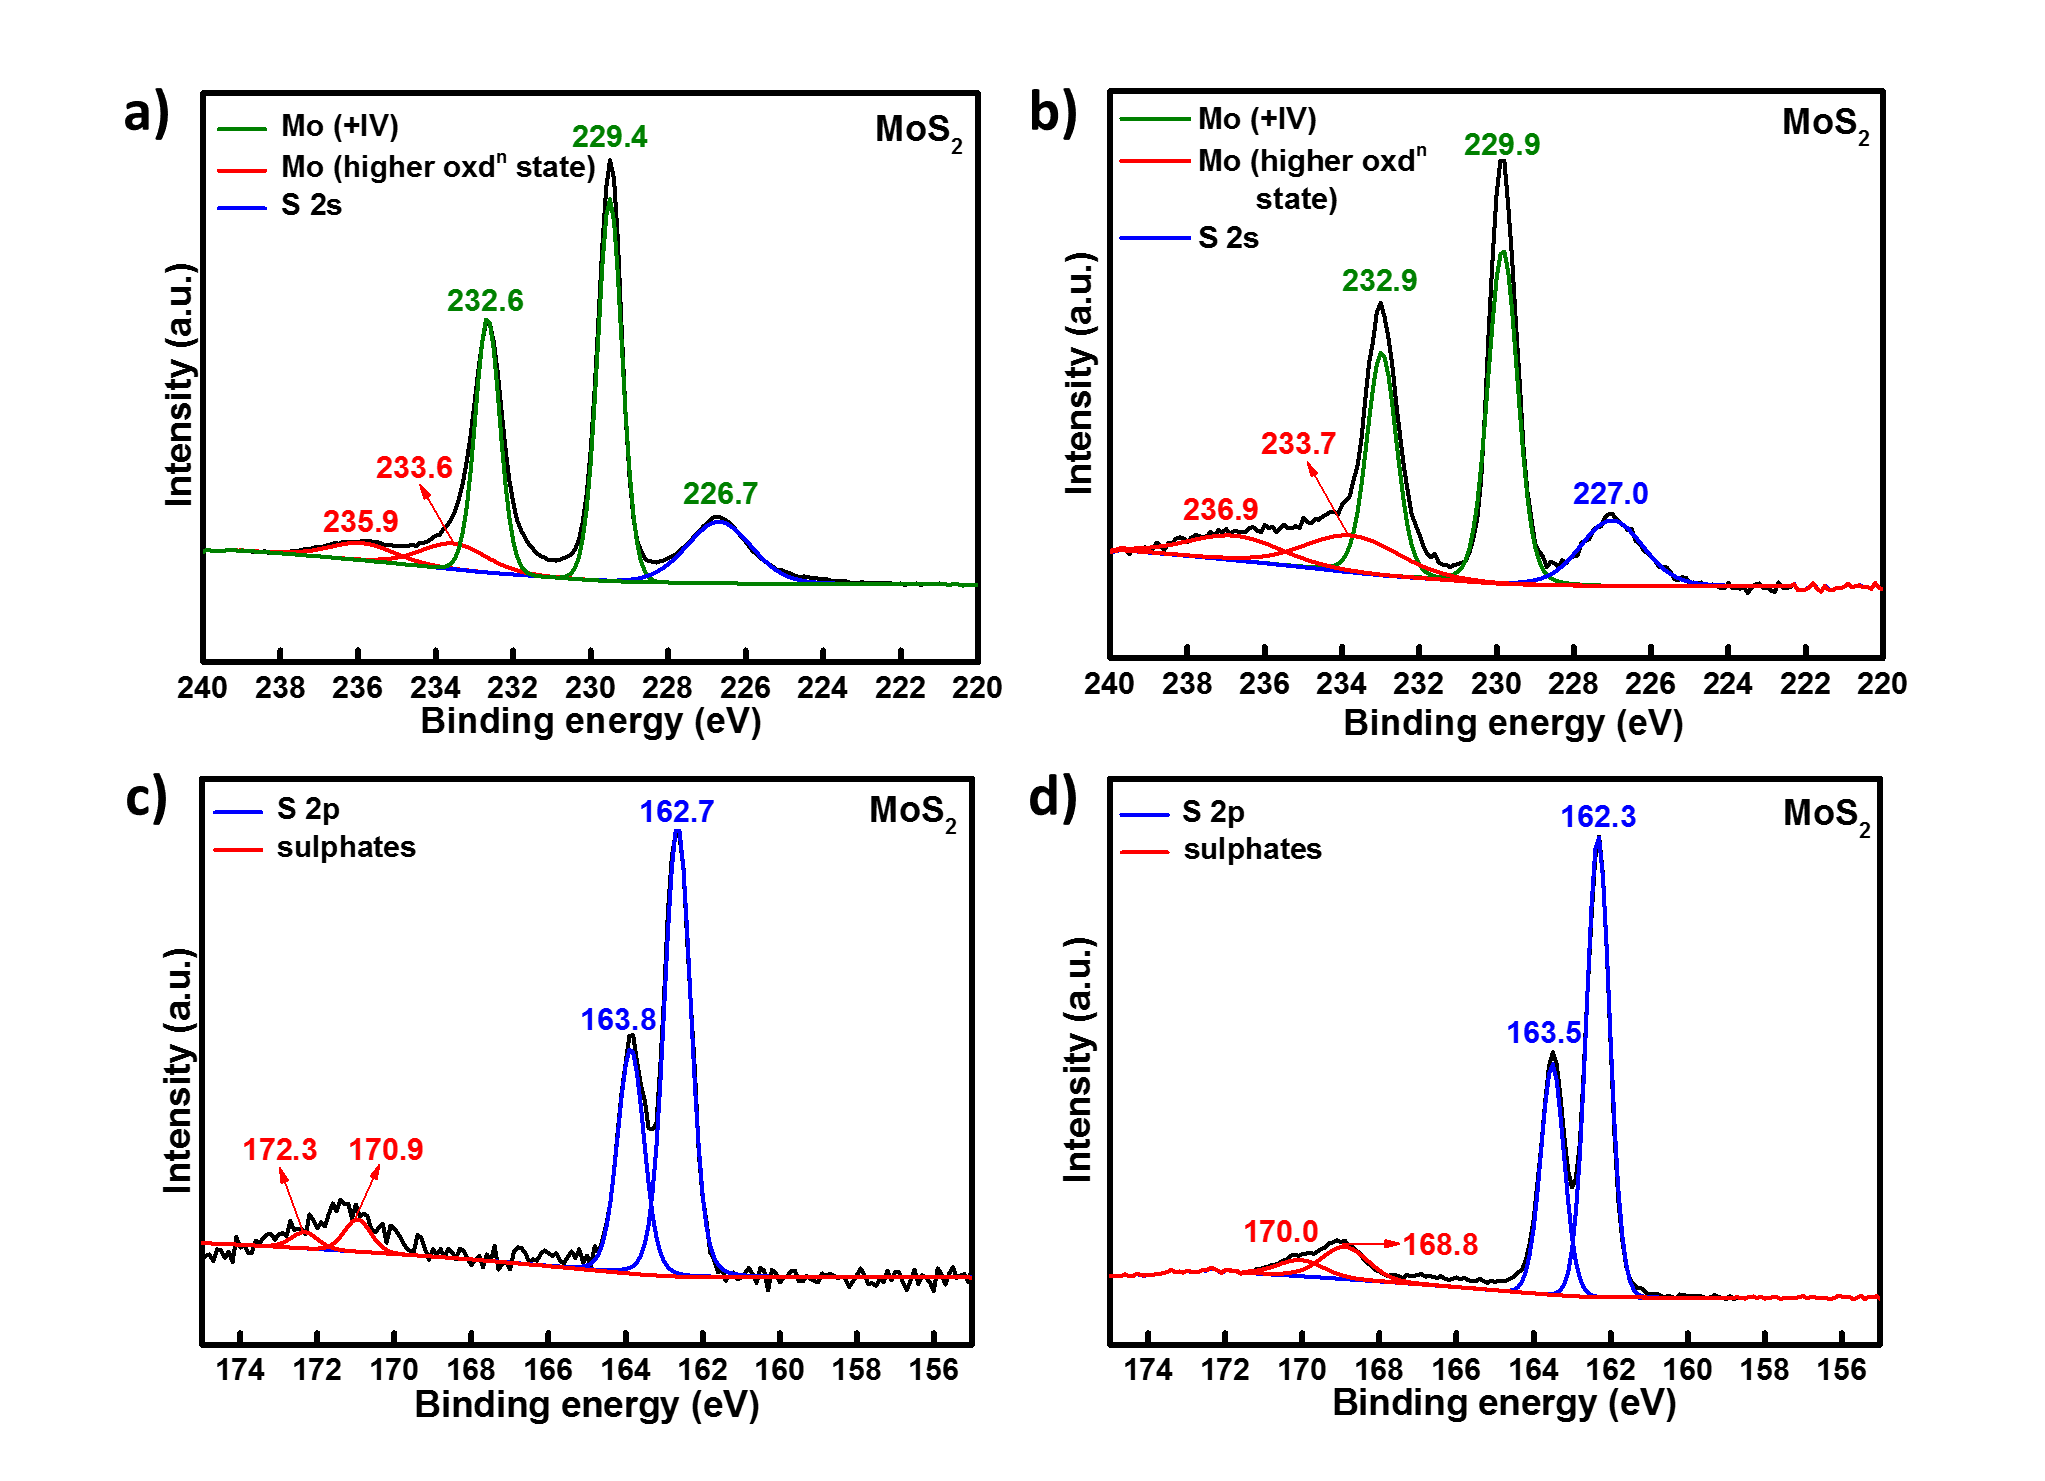
\includegraphics[width=\textwidth]{Figures/appendix/MoS2XPS}
  \caption{XPS spectra of Mo 3d orbitals in a a) pristine and b) charged \ce{MoS2} cathode and binding energies of S 2p orbital in a a) pristine and b) charged \ce{MoS2} cathode.}
  \label{Figures/appendix:MoS2XPS}
\end{figure}
\begin{figure}[tbh!]
\centering
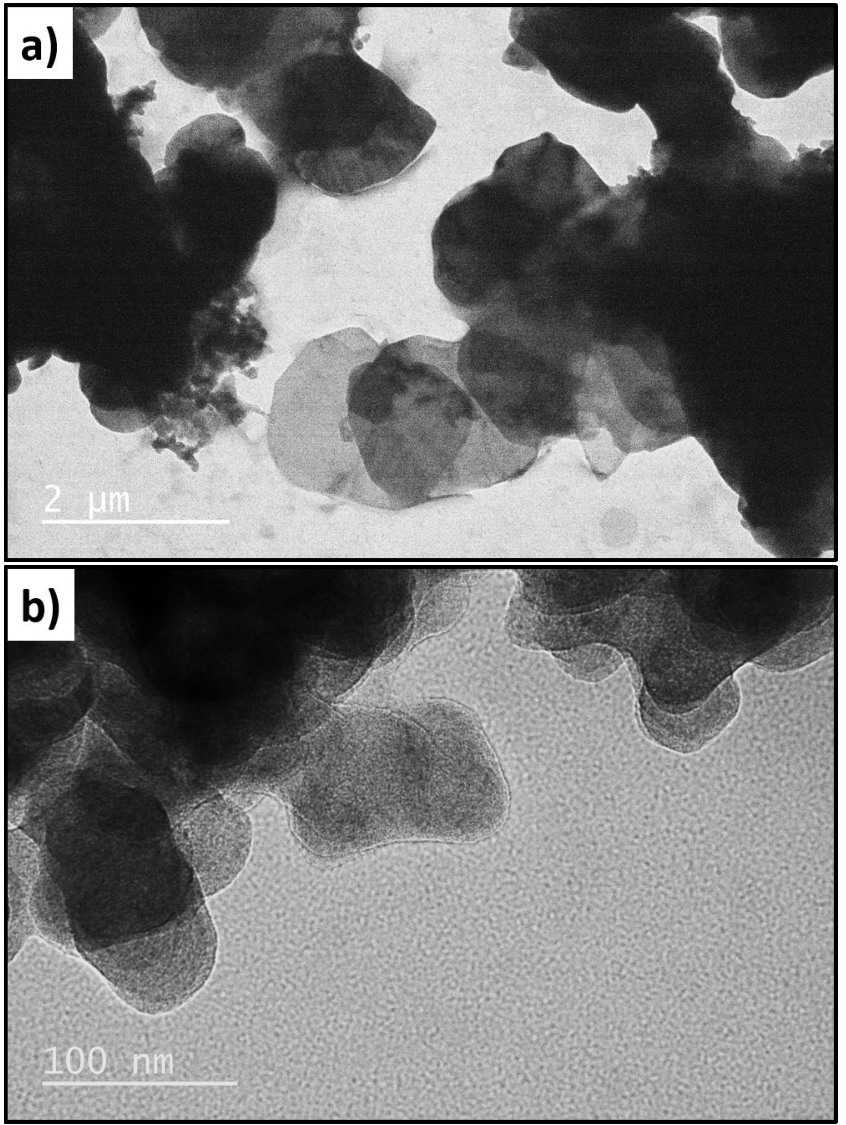
\includegraphics[width=\textwidth]{Figures/appendix/hbntem.pdf}
\caption{TEM micrographs of h-BN displaying the hexagonal layered structure.}
\label{Figures/appendix:hbntem}
\end{figure}
\begin{figure}[tbh!]
\centering
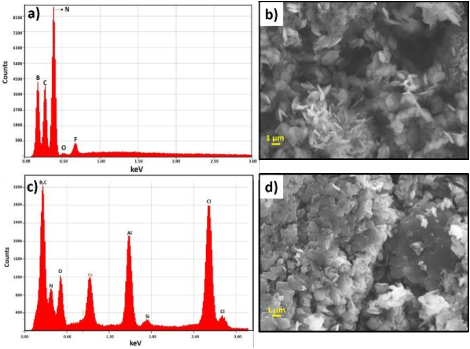
\includegraphics[width=\textwidth]{Figures/appendix/hbnedxsem.pdf}
\caption{a) EDXS profile and b) SEM image of a pristine h-BN cathode. c) EDXS profile and d) SEM image of a cycled h-BN cathode. The cycled cathode shows agglomeration and its EDXS spectra contains peaks of both aluminium and chlorine.}
\label{Figures/appendix:hbnedxsem}
\end{figure}
\begin{figure}[tbh!]
\centering
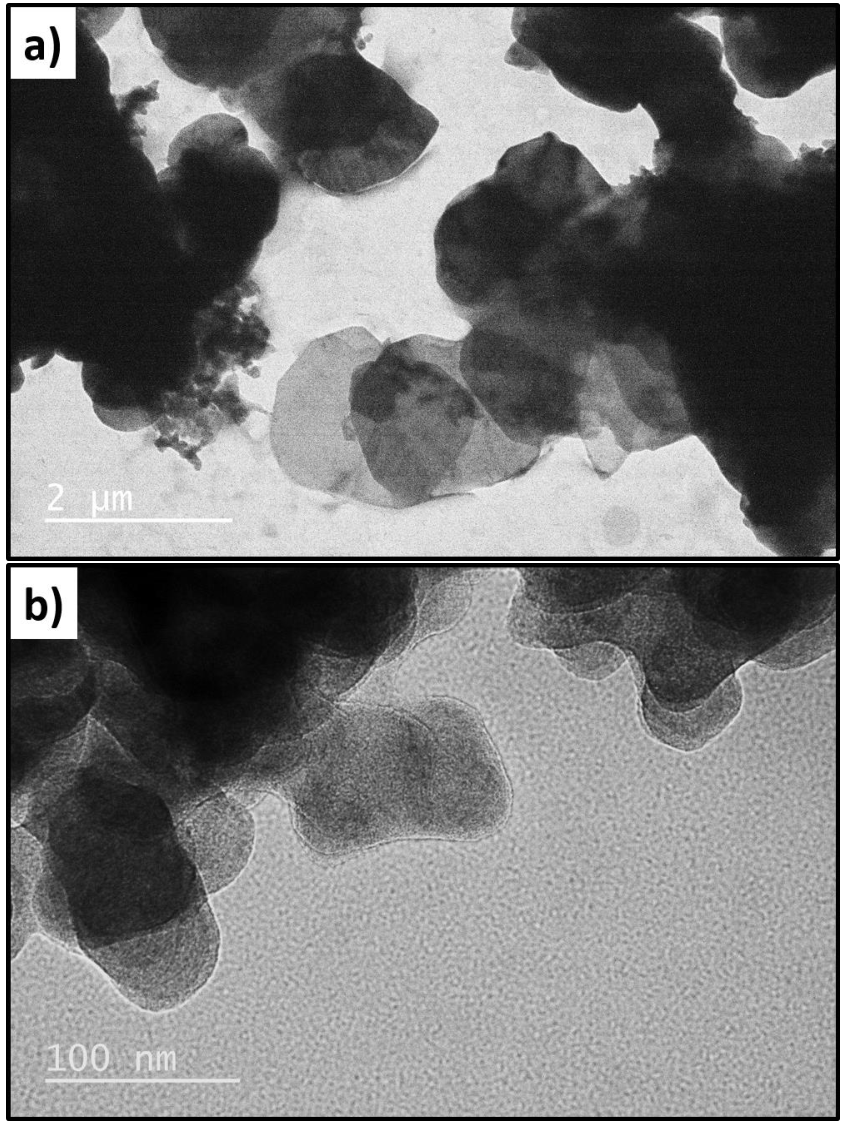
\includegraphics[width=\textwidth]{Figures/appendix/cntem.pdf}
\caption{TEM micrographs of g-\ce{C3N4} showing presence of different lattice fringes, which confirm presence of crystallinity.}
\label{Figures/appendix:cntem}
\end{figure}